\documentclass[journal,12pt,twocolumn]{IEEEtran}

\usepackage{setspace}
\usepackage{gensymb}
\singlespacing
\usepackage[cmex10]{amsmath}

\usepackage{amsthm}

\usepackage{mathrsfs}
\usepackage{txfonts}
\usepackage{stfloats}
\usepackage{bm}
\usepackage{cite}
\usepackage{cases}
\usepackage{subfig}

\usepackage{longtable}
\usepackage{multirow}

\usepackage{enumitem}
\usepackage{mathtools}
\usepackage{steinmetz}
\usepackage{tikz}
\usepackage{circuitikz}
\usepackage{verbatim}
\usepackage{tfrupee}
\usepackage[breaklinks=true]{hyperref}
\usepackage{graphicx}
\usepackage{tkz-euclide}

\usetikzlibrary{calc,math}
\usepackage{listings}
    \usepackage{color}                                            %%
    \usepackage{array}                                            %%
    \usepackage{longtable}                                        %%
    \usepackage{calc}                                             %%
    \usepackage{multirow}                                         %%
    \usepackage{hhline}                                           %%
    \usepackage{ifthen}                                           %%
    \usepackage{lscape}     
\usepackage{multicol}
\usepackage{chngcntr}

\DeclareMathOperator*{\Res}{Res}

\renewcommand\thesection{\arabic{section}}
\renewcommand\thesubsection{\thesection.\arabic{subsection}}
\renewcommand\thesubsubsection{\thesubsection.\arabic{subsubsection}}

\renewcommand\thesectiondis{\arabic{section}}
\renewcommand\thesubsectiondis{\thesectiondis.\arabic{subsection}}
\renewcommand\thesubsubsectiondis{\thesubsectiondis.\arabic{subsubsection}}


\hyphenation{op-tical net-works semi-conduc-tor}
\def\inputGnumericTable{}                                 %%

\lstset{
%language=C,
frame=single, 
breaklines=true,
columns=fullflexible
}
\begin{document}


\newtheorem{theorem}{Theorem}[section]
\newtheorem{problem}{Problem}
\newtheorem{proposition}{Proposition}[section]
\newtheorem{lemma}{Lemma}[section]
\newtheorem{corollary}[theorem]{Corollary}
\newtheorem{example}{Example}[section]
\newtheorem{definition}[problem]{Definition}

\newcommand{\BEQA}{\begin{eqnarray}}
\newcommand{\EEQA}{\end{eqnarray}}
\newcommand{\define}{\stackrel{\triangle}{=}}
\bibliographystyle{IEEEtran}
\raggedbottom
\setlength{\parindent}{0pt}
\providecommand{\mbf}{\mathbf}
\providecommand{\pr}[1]{\ensuremath{\Pr\left(#1\right)}}
\providecommand{\qfunc}[1]{\ensuremath{Q\left(#1\right)}}
\providecommand{\sbrak}[1]{\ensuremath{{}\left[#1\right]}}
\providecommand{\lsbrak}[1]{\ensuremath{{}\left[#1\right.}}
\providecommand{\rsbrak}[1]{\ensuremath{{}\left.#1\right]}}
\providecommand{\brak}[1]{\ensuremath{\left(#1\right)}}
\providecommand{\lbrak}[1]{\ensuremath{\left(#1\right.}}
\providecommand{\rbrak}[1]{\ensuremath{\left.#1\right)}}
\providecommand{\cbrak}[1]{\ensuremath{\left\{#1\right\}}}
\providecommand{\lcbrak}[1]{\ensuremath{\left\{#1\right.}}
\providecommand{\rcbrak}[1]{\ensuremath{\left.#1\right\}}}
\theoremstyle{remark}
\newtheorem{rem}{Remark}
\newcommand{\sgn}{\mathop{\mathrm{sgn}}}
% \providecommand{\abs}[1]{\left\vert#1\right\vert}
% \providecommand{\res}[1]{\Res\displaylimits_{#1}} 
% \providecommand{\norm}[1]{\left\lVert#1\right\rVert}
% %\providecommand{\norm}[1]{\lVert#1\rVert}
% \providecommand{\mtx}[1]{\mathbf{#1}}
% \providecommand{\mean}[1]{E\left[ #1 \right]}
\providecommand{\fourier}{\overset{\mathcal{F}}{ \rightleftharpoons}}
%\providecommand{\hilbert}{\overset{\mathcal{H}}{ \rightleftharpoons}}
\providecommand{\system}{\overset{\mathcal{H}}{ \longleftrightarrow}}
	%\newcommand{\solution}[2]{\textbf{Solution:}{#1}}
\newcommand{\solution}{\noindent \textbf{Solution: }}
\newcommand{\cosec}{\,\text{cosec}\,}
\providecommand{\dec}[2]{\ensuremath{\overset{#1}{\underset{#2}{\gtrless}}}}
\newcommand{\myvec}[1]{\ensuremath{\begin{pmatrix}#1\end{pmatrix}}}
\newcommand{\mydet}[1]{\ensuremath{\begin{vmatrix}#1\end{vmatrix}}}
\numberwithin{equation}{subsection}
\makeatletter
\@addtoreset{figure}{problem}
\makeatother
\let\StandardTheFigure\thefigure
\let\vec\mathbf
\renewcommand{\thefigure}{\theproblem}
\def\putbox#1#2#3{\makebox[0in][l]{\makebox[#1][l]{}\raisebox{\baselineskip}[0in][0in]{\raisebox{#2}[0in][0in]{#3}}}}
     \def\rightbox#1{\makebox[0in][r]{#1}}
     \def\centbox#1{\makebox[0in]{#1}}
     \def\topbox#1{\raisebox{-\baselineskip}[0in][0in]{#1}}
     \def\midbox#1{\raisebox{-0.5\baselineskip}[0in][0in]{#1}}
\vspace{3cm}
\title{Assignment 1}
\author{Ganraj Borade - EE18BTECH11016}
\maketitle
\newpage
\bigskip
\UseRawInputEncoding
\renewcommand{\thefigure}{\theenumi}
\renewcommand{\thetable}{\theenumi}
Download all Codes from 
%
\begin{lstlisting}
https://github.com/ganrajborade/EE4013_C-DS/blob/main/codes/
\end{lstlisting}

\section{Problem}
Q.35 Consider the following ANSI C Program.
\begin{lstlisting}
#include <stdio.h>
#include <stdlib.h>
struct Node{
	int value;
	struct Node *next;};
int main(){
    struct Node *boxE, *head, *boxN; int index = 0;
    boxE=head= (struct Node *) malloc(sizeof(struct Node));
    head->value = index;
    for (index =1; index<=3; index++){
	    boxN = (struct Node *) malloc (sizeof(struct Node));
	    boxE->next = boxN;
	    boxN->value = index;
	    boxE = boxN; }
    for (index=0; index<=3; index++) {
	    printf(“Value at index %d is %d\n”, index, head->value);
	    head = head->next;
	    printf(“Value at index %d is %d\n”, index+1, head->value); }
}
\end{lstlisting}
 Which one of the following statements below is correct about the program?

\section{Solution}
\textbf{Answer} : It dereferences an uninitialized pointer that may result in a run-time error
\newline

\textbf{Explanation}
\begin{lstlisting}
struct Node{
	int value;
	struct Node *next;};
\end{lstlisting}
	The above structure is for linked list node.
Let's now look at the main function in the given code :
\begin{lstlisting}
struct Node *boxE, *head, *boxN; int index = 0;
\end{lstlisting}
i.e there are 3 pointers : boxE, head and boxN. Now since these pointer variables are not initialized to null so they will point to some unwanted memory location. And we also have variable 'index'=0
\newline
\begin{lstlisting}
boxE=head= (struct Node *) malloc(sizeof(struct Node));
head->value = index;
\end{lstlisting}
Now we are going to assign boxE equal to head and then we are allocating the memory of size struct Node. So here a dynamic memory allocation will happen and a node will be created in a heap area.
\begin{figure}[!h]
	\centering
	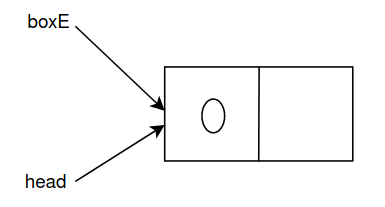
\includegraphics[width=\columnwidth]{./figs/1.png}
\end{figure}

i.e boxE and head will be pointing to this node created and in this node for now garbage value is present. Since we are doing head $\rightarrow$ value = index so, data value for this head is 0 as index is 0 now. And the next pointer will point to garbage location.
\newline
\begin{lstlisting}
for (index =1; index<=3; index++){
	boxN = (struct Node *) malloc (sizeof(struct Node));
	boxE->next = boxN;
	boxN->value = index;
	boxE = boxN; }
\end{lstlisting}
\textbf{1.}
\newline
In the above for loop, initially index=1. The output of 1st iteration is as follows :
\begin{figure}[!h]
	\centering
	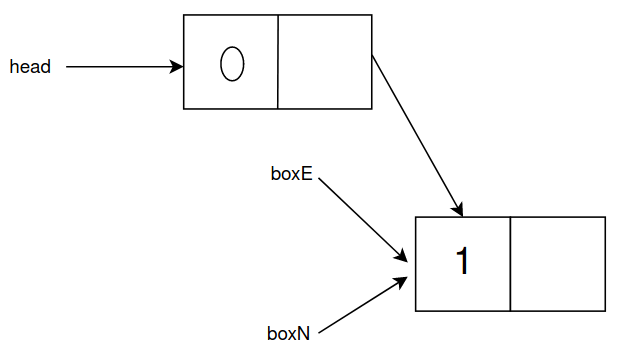
\includegraphics[width=\columnwidth]{./figs/2.png}
\end{figure}

Because a new node boxN will be created as the loop runs. And since we are doing boxE$\rightarrow$next = boxN so as shown in the above figure, the next of boxE will point to boxN. After that since boxN$\rightarrow$value = index, so boxN value will be equal to 1 and after that since boxE= boxN, so again boxE will be pointing to boxN.
\newline
\textbf{2.}
\newline
Similarly after 3 iterations, we will get following output in the node form :
\begin{figure}[!h]
	\centering
	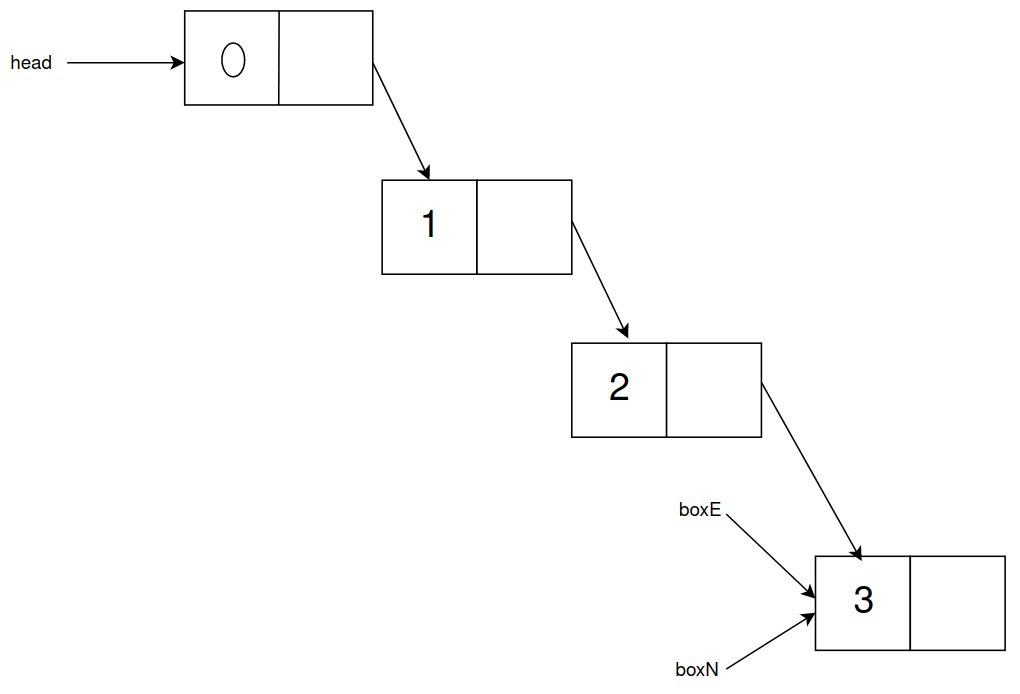
\includegraphics[width=\columnwidth]{./figs/3.png}
\end{figure}
\newline

\begin{lstlisting}
for (index=0; index<=3; index++) {
	printf(“Value at index %d is %d\n”, index, head->value);
	head = head->next;
	printf(“Value at index %d is %d\n”, index+1, head->value); }
\end{lstlisting}
Now we can easily look at the output now. 
\textbf{1.}
\newline
When index=0, then we will get output as :
\newline
Value at index 0 is 0
\newline 
Value at index 1 is 1 
\newline
Because in the second line of above code (head = head$\rightarrow$next), we will get head pointed to value 1.
\newline
\newline
Similarly at index=1, we will get :
\newline
Value at index 1 is 1
\newline 
Value at index 2 is 2 
\newline
\newline

Similarly at index=2, we will get :
\newline
Value at index 2 is 2
\newline 
Value at index 3 is 3 
\newline
\newline
Now when index=3, firstly we will get :
\newline
Value at index 3 is 3 
\newline
Now head = head$\rightarrow$next, but now, head$\rightarrow$next is some unwanted pointer so it will contain some pointer to some garbage location therfore when head$\rightarrow$value will run, we could get a segmentation fault here because we are accessing an unwanted address.So, this program will be abnormally terminated.
\newline
Hence the answer is "It dereferences an uninitialized pointer that may result in a run-time error"
\newline
\newline
The correct code of the program will be :
\begin{lstlisting}
#include <stdio.h>
#include <stdlib.h>
struct Node{
int value;
struct Node *next;};
int main(){
struct Node *boxE, *head, *boxN; int index = 0;
boxE=head= (struct Node *) malloc(sizeof(struct Node));
head->value = index;
for (index =1; index<=3; index++){
boxN = (struct Node *) malloc (sizeof(struct Node));
boxE->next = boxN;
boxN->value = index;
boxE = boxN; }
for (index=0; index<=2; index++) {
printf(“Value at index %d is %d\n”, index, head->value);
head = head->next;
printf(“Value at index %d is %d\n”, index+1, head->value); }
}

\end{lstlisting}
That is in the last for loop just reduce last value of index to 2.
\end{document}
